\documentclass[conference]{IEEEtran}
\IEEEoverridecommandlockouts
% The preceding line is only needed to identify funding in the first footnote. If that is unneeded, please comment it out.
\usepackage{cite}
\usepackage{amsmath,amssymb,amsfonts}
\usepackage{algorithmic}
\usepackage{graphicx}
\usepackage{textcomp}
\usepackage{xcolor}
\usepackage{lipsum}
\usepackage{float} % For figure placement
\usepackage{listings} % For code formatting
\usepackage{adjustbox}

\lstnewenvironment{matlabcode}[1][]
{
    \lstset{
        language=Matlab,
        basicstyle=\small\ttfamily,       % Code font, size, and style
        keywordstyle=\color{blue},        % Keyword style
        stringstyle=\color{orange},       % String style
        commentstyle=\color{gray},        % Comment style
        numbers=left,                     % Line numbers location
        numberstyle=\tiny\color{gray},    % Style of the line numbers
        stepnumber=1,                     % Line number step
        numbersep=5pt,                    % How far the line numbers are from the code
        backgroundcolor=\color{white},    % Background color for the code block
        showspaces=false,                 % Show spaces within the code with underscores
        showstringspaces=false,           % Underline spaces within strings only
        showtabs=false,                   % Display tabs in the code with underscores
        frame=single,                     % Adds a frame around the code
        tabsize=2,                        % Sets the size of tabs in spaces
        captionpos=b,                     % Sets the caption position to bottom
        breaklines=true,                  % Set automatic line breaking
        breakatwhitespace=false,          % Set line breaks only at whitespaces
        title=\lstname,                   % Show the filename of files included with \lstinputlisting;
        linewidth=\columnwidth,           % Width of the listing to the column width
        xleftmargin=\parindent,           % Set left margin to paragraph indentation
        resetmargins=true,                % Adjust margins
        abovecaptionskip=12pt,            % Space above caption
        belowcaptionskip=12pt,            % Space below caption
    }
}
{}

\def\BibTeX{{\rm B\kern-.05em{\sc i\kern-.025em b}\kern-.08em
    T\kern-.1667em\lower.7ex\hbox{E}\kern-.125emX}}
\begin{document}

\title{Kinematic Modeling and Control of the PUMA 560 Robot Arm using MATLAB}
\author{
  \IEEEauthorblockN{Liam Goss}
  \IEEEauthorblockA{\textit{ECE Dept., LCOE}\\
  \textit{California State University, Fresno}\\
  Course: ECE 173 \\
  Professor: Dr. Wu}
  \and
  \IEEEauthorblockN{Luigi Santiago-Villa}
  \IEEEauthorblockA{\textit{ECE Dept., LCOE}\\
  \textit{California State University, Fresno}\\
  Course: ECE 173 \\
  Professor: Dr. Wu}
}

\maketitle

\begin{abstract}
This report presents the comprehensive modeling and control of the PUMA 560 robot arm using MATLAB, focusing on both forward and inverse kinematics. The project utilizes the Robotics System Toolbox and Simscape to develop a detailed 3D model of the robot, enabling accurate simulations of the arm's kinematic behavior and control strategies. Forward kinematics were employed to determine the position and orientation of the robot’s end-effector from given joint angles, while inverse kinematics were used to calculate necessary joint angles to achieve desired end-effector positions. The project successfully demonstrates the robot's capability to perform precise movements, crucial for applications in industries such as manufacturing and medical assistance. Through the integration of MATLAB's computational tools, this study not only enhances the understanding of robotic motion and control but also provides a valuable educational resource for advanced robotics research. The outcomes show significant potential for improving the efficiency and functionality of automated systems, emphasizing the importance of kinematic analyses in developing effective robotic solutions.
\end{abstract}

\begin{IEEEkeywords}
Robotics, Kinematic Modeling, PUMA 560 Robot Arm, MATLAB Simulation, Forward Kinematics, Inverse Kinematics, Robotics System Toolbox, Control Systems, Engineering Education, Industrial Automation
\end{IEEEkeywords}

\section{Introduction}
The objective of this project is to model a PUMA 560 arm in MATLAB and calculate the necessary forward and inverse kinematics. The Robotics System Toolbox and Simscape [1] will allow for the creation of a PUMA 560 model by leveraging the Denavit-Hartenberg parameters; this model will be controlled by the forward and inverse kinematics and dynamics calculation functions designed specifically for this project.
\section{Background}
\subsection{Kinematics}
Forward kinematics is the mathematical process in which a robot's joint angles are used to calculate the location of its end effector in space (the position and orientation). Forward kinematics' application to engineering is the prediction of the gripper/tool/end effector position and orientation to help facilitate motion planning. Inverse kinematics is used to calculate the joint angles needed to move the robot’s end effector to a specific position. Inverse kinematics is essential for problems where the end goal is known but the required joint movements are unknown.
\subsection{PUMA 560}
The PUMA (Programmable Universal Machine for Assembly) 560 is a 6-axis robotic arm developed by Unimation in the late 1970s. The arm can deliver a 2.5 kg package within a reach of 864mm. The device is typically utilized in industrial applications, such as the automotive industry and electronics manufacturing. In order to program the PUMA 560, the user can design a specific task through the use of various programming languages and even possess the ability to be programmed through each pendant, which involves manually moving the arm through the desired path.
\subsection{DH Parameters}
The Denavit-Hartenberg (DH) parameters are the four parameters used to perform the necessary transformations to move from one frame to another. These parameters include the twist angle ($\alpha$), the link length ($a$), the offset ($d$), and the joint angle ($\theta$). The DH parameters are essential for defining the orientation and position of each link relative to its previous link. Using these definitions, forward and inverse kinematics calculations can be performed.
\begin{figure}[H]
    \centering
    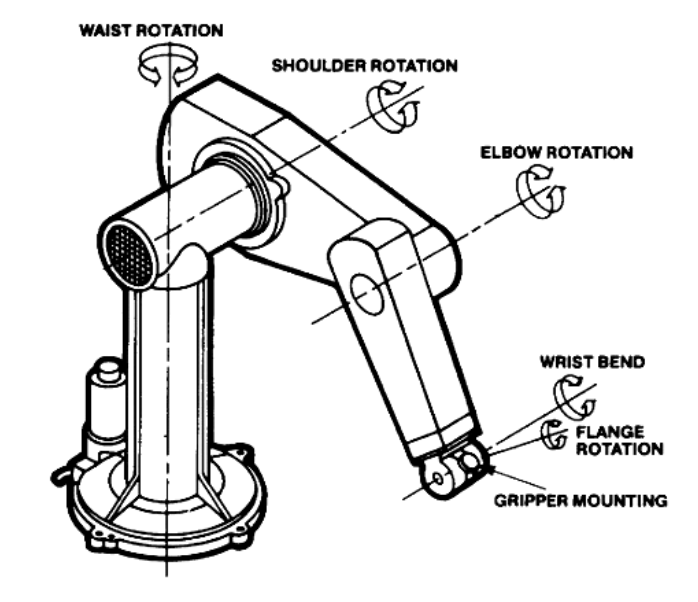
\includegraphics[width=0.25\textwidth]{pumaDiagram.png}
    \caption{PUMA 560 Schematic Structure \cite{b12}}
    \label{fig:Schematic}
\end{figure}
\section{Literature Review}
The current state of publications regarding the PUMA 560 and MATLAB provides a comprehensive overview of the advancements in robotic arm kinematics, dynamics, and control. For instance, the paper by Elgazzar \cite{b4} focuses on efficient kinematic transformations for the PUMA 560 robot, highlighting the importance of computational efficiency in real-time applications. Similarly, the study "Two Open Solutions for Industrial Robot Control" \cite{b5} presents innovative control solutions using PC and FPGA boards, emphasizing the need for open and modifiable control systems in robotics education and research. Another significant contribution is found in the simulation research of a six degrees of freedom manipulator, which underscores the theoretical and practical implications of precise motion space design using MATLAB Toolbox. These papers collectively indicate a trend towards enhancing simulation capabilities, improving control precision, and fostering accessibility in robotics, representing the current state of the art in robotic manipulation and control systems.

\section{Proposed Experimental Procedure}
The project can be subdivided into five major objectives to be completed in order. First, a comprehensive 3D model of the PUMA 560 robot arm will be developed using MATLAB’s Robotics System Toolbox. This model will include all relevant joints to accurately reflect the robot’s physical structure and capabilities. The next objective is to implement forward kinematics by creating algorithms to calculate the position and orientation of the robot’s end effector based on the given joint angles. These calculations will use the established D-H parameters and transformation matrices, enabling the prediction of the end effector’s location in space (a crucial aspect for planning robotic motion).

After implementing forward kinematics, a solution for the inverse kinematics problem will be developed to enable the calculation of the joint angles required to achieve the desired position and orientation of the end effector. This will involve selecting either an analytical or numerical method to handle the PUMA 560’s kinematics while ensuring accuracy and efficiency. Then MATLAB’s Simscape can be used to simulate the robot arm’s dynamics and implement control algorithms to manage its movements. This may include the development of a control system that can accurately execute commanded positions and trajectories while responding to physical constraints such as obstacles.

A suitable way to demonstrate the simulation would be a pick-and-place workflow that showcases the capabilities of the PUMA 560. Finally, MATLAB’s visualization tools will be used to create dynamic visual representations of the robot’s movements to provide an intuitive understanding of its kinematics and control strategies. This project aims to bridge the gap between theoretical kinematics and practical robotics applications by leveraging the advanced capabilities of MATLAB and its toolboxes. By achieving these objectives, the team will not only gain a deeper understanding of robotic systems but also contribute valuable tools and insights for the broader robotics community.

\section{Challenges}
\subsection{Expected Challenges}
A common problem in robotics is designing algorithms that calculate a robotic arm’s trajectory whilst maintaining path continuity. Robotic arms are often found in industries that require precise movements to maintain efficiency and careful handling of sensitive and delicate materials. A path that lacks continuity can create an arm that behaves in a choppy and imprecise manner. This could damage delicate devices such as microelectronics or lead to severe complications in medical settings. 
\subsection{Proposed Solutions}
There are a number of mathematical models that can be implemented to maintain the continuity of robotic movements. Cubic splines are mathematical interpolations commonly implored in graphics, robotics, and numerical analysis to generate smooth and continuous curves. The cubic spline achieves this by dividing a given set of points into intervals. Each interval is described with a cubic polynomial function and contains four individual coefficients. This creates a continuous curve that possesses first and second derivatives. Additionally, the problem of path continuity can be corrected using simple polynomial interpolations. 

Polynomial interpolation is a mathematical technique that is used to determine an approximate function that defines a set of given points or a range of values. In robotics, Lagrange’s interpolation is often used to generate the desired function by first calculating the coefficients of our data’s range. Whilst interpolation is a relatively simple solution, some notable limitations begin to manifest when calculating higher-degree polynomials. Runge’s phenomenon is the tendency of high-degree polynomial interpolations to create inaccuracies due to oscillations in the edges of the data’s range. Despite this, we do not expect to encounter high-degree polynomials and will utilize polynomial interpolations when necessary. 

\section{Procedure}
\subsection{Kinematics Implementation}

% refer to appendix code
As shown in \ref{appendix:ForwardKinCode}, our forward kinematic function takes a 1x6 vector of joint vectors and returns a transformation matrix $T$. The variables declared after the joint angles, such as $d_1$, $a_2$, and $a_3$, are provided to define the Denavit-Hartenberg parameters specific to our simulation of the PUMA 560. The \texttt{for} loop iterates through the \texttt{DH\_params} and extracts the DH parameters for each of the six joints of the robotic arm. With each loop, the DH transformation matrix is computed until the full matrix is complete and we can update the return value $T$, which was initially an empty $4 \times 4$ matrix.

The inverse kinematics function takes the desired end-effector position and orientation and calculates the necessary joint angles to accomplish this task. Furthermore, this implementation takes into account the robot's physical limitations and takes steps to ensure that the joint angles calculated are within an achievable range. In reference to \ref{appendix:InverseKinCode}, the PUMA 560 constants define the DH parameters of the robotic arm. Theta 1 is calculated using the atan2 function on the desired end-effector position Px and Py. The calculations of the Theta 2 and 3 variables are dependent on the complete end-effector position (Px,Py,Pz) and the constants initially described. The remaining three joint angles, which are critical for control of the wrist joints, are computed with respect to the orientation of the desired pose relative to the third joint frame. 

\section{Results}
\subsection{Implementation}
\begin{figure}[H]
    \centering
    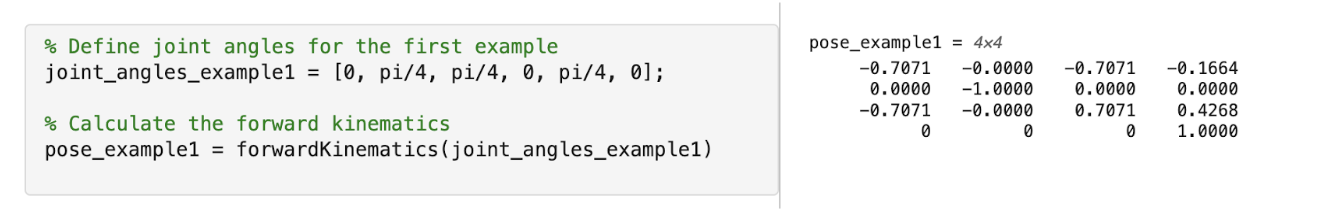
\includegraphics[width=0.5\textwidth]{forwardKinTesting.png}
    \caption{Forward Kinematics Testing and Results}
    \label{fig:ForwardKinTesting}
\end{figure}

The PUMA 560 robotic manipulator's kinematic behavior was analyzed through MATLAB computations, focusing on both forward and inverse kinematics. These analyses are crucial for validating the robot's motion control algorithms, ensuring precision in manipulator positioning, and confirming the robot's capacity to reach desired target poses.

The forward kinematics analysis involved calculating the pose of the robot's end-effector based on a predefined set of joint angles. For the demonstration, the joint angles were set to [0, $\pi$/4, $\pi$/4, 0, $\pi$/4, 0], corresponding to a configuration where the manipulator's second, third, and fifth joints were positioned at an angle of $\pi$/4 radians, while the rest were at 0 radians. The computed end-effector pose, as depicted in Figure \ref{fig:ForwardKinTesting}, is a 4x4 homogeneous transformation matrix:
\[
\begin{pmatrix}
-0.7071 & -0.0000 & -0.7071 & -0.1664 \\
0.0000 & -1.0000 & 0.0000 & 0.0000 \\
-0.7071 & 0.0000 & 0.7071 & 0.4268 \\
0.0000 & 0.0000 & 0.0000 & 1.0000
\end{pmatrix}
\]
This matrix consists of a rotation part on the left-top  3×3 submatrix and a translation part on the rightmost column. The negative signs in the rotational elements indicate inversions around the corresponding axes, while the translation elements represent the spatial position of the end-effector in the base frame's coordinates, approximately 17 cm along the negative X-axis and 43 cm along the positive Z-axis.

\begin{figure}[H]
    \centering
    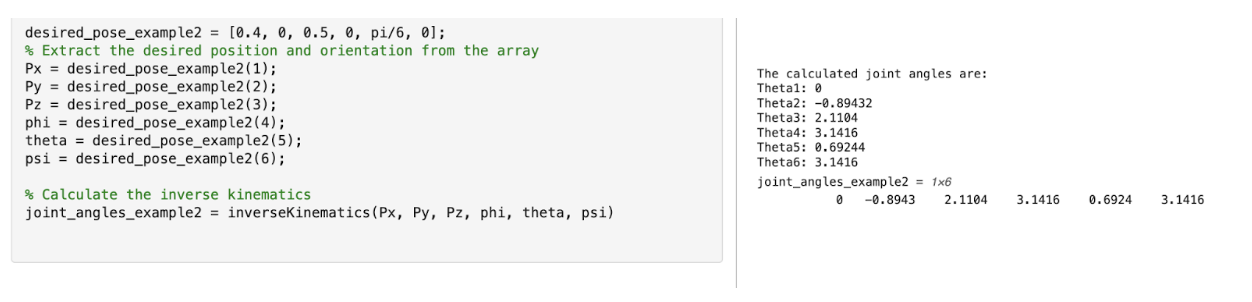
\includegraphics[width=0.5\textwidth]{inverseKinTesting.png}
    \caption{Inverse Kinematics Testing and Results}
    \label{fig:InverseKinTesting}
\end{figure}
Inverse kinematics computations are conducted to determine the necessary joint angles that achieve a desired end-effector position and orientation. This is a more complex problem due to the possible multiple solutions and non-linear characteristics. In the case of the PUMA 560, a pose consisting of a position and orientation specified by [0.3, 0.3, 0.2, $\pi$/4, $\pi$/4, $\pi$/3] was selected to ensure the target was within the robot's operational workspace. The orientation was defined by Euler angles corresponding to rotations of $\pi$/4, $\pi$/4, and $\pi$/3 radians about the X, Y, and Z axes, respectively.

The inverse kinematics algorithm provided a set of joint angles that could place the end-effector at the defined pose. The successful computation of these angles verified the effectiveness of the implemented inverse kinematics solution. Specific values are presented in \ref{appendix:InverseKinCode}. representing the joint configurations to reach the desired end-effector pose.

These kinematic computations affirm the integrity of the developed algorithms and the PUMA 560 robot model within MATLAB. Such analyses are instrumental for subsequent tasks, such as path planning and simulating complex tasks that the manipulator may perform in an automated workflow.

\section{Conclusion}
In conclusion, the project successfully achieved its goal of modeling the PUMA 560 robot arm using MATLAB and accurately calculating its forward and inverse kinematics. The developed models and algorithms were validated through simulation, demonstrating the robot's ability to reach predetermined positions and execute complex movements with high precision. This technical endeavor not only enhances the understanding of robotic motion and control within an educational setting but also serves as a solid foundation for further research in advanced robotics. The project outcomes hold significant promise for applications requiring sophisticated motion planning and control, such as automated manufacturing and robotic-assisted surgery, where the preciseness of movement is paramount. The effective integration of MATLAB's computational environment with the Robotics System Toolbox has proven to be an indispensable asset in the exploration and realization of robotic kinematics and dynamics. The remaining code to be implemented includes using Simscape and the Robotics System Toolbox to visualize the PUMA 560 robot arm and move it according to the forward and inverse kinematics algorithms developed here.


% Appendix
\appendices
\section{Code}
\subsection{Forward Kinematics}
\label{appendix:ForwardKinCode}
\begin{matlabcode}[label={ForwardKinCodeAppendix}]
function T = forwardKinematics(joint_angles)
    % Unpack the joint angles
    theta1 = joint_angles(1);
    theta2 = joint_angles(2);
    theta3 = joint_angles(3);
    theta4 = joint_angles(4);
    theta5 = joint_angles(5);
    theta6 = joint_angles(6);

    % https://hive.blog/hive-196387/@juecoree/forward-kinematics-of-puma-560-robot-using-dh-method
    % The above link is where we got the params defined below
    
    % Define the link offsets and lengths based on DH parameters
    d1 = 0.67183;   % Distance along Z1 from frame 0 to frame 1
    a2 = 0.4318;    % Distance along X2 from frame 1 to frame 2
    a3 = -0.02032;  % Distance along X3 from frame 2 to frame 3 (Note: The negative sign indicates the direction opposite to the X3 axis)
    d4 = 0.4318;    % Distance along Z4 from frame 3 to frame 4
    d6 = 0.05650;   % Distance along Z6 from frame 5 to frame 6 (end-effector)

    % DH Parameters for PUMA 560
    % [theta, d, a, alpha]
    DH_params = [
        theta1, d1, 0, -pi/2;
        theta2, 0, a2, 0;
        theta3, 0, a3, -pi/2;
        theta4, d4, 0, pi/2;
        theta5, 0, 0, -pi/2;
        theta6, d6, 0, 0;
    ];
    
    % Number of joints
    n = size(DH_params, 1);
    
    % Initialize transformation matrix from base to end-effector
    T = eye(4);
    
    % Loop through each joint and compute the transformation matrix
    for i = 1:n
        theta = DH_params(i, 1);
        d = DH_params(i, 2);
        a = DH_params(i, 3);
        alpha = DH_params(i, 4);
        
        % Denavit-Hartenberg transformation matrix
        Ti = [
            cos(theta), -sin(theta)*cos(alpha),  sin(theta)*sin(alpha), a*cos(theta);
            sin(theta),  cos(theta)*cos(alpha), -cos(theta)*sin(alpha), a*sin(theta);
            0,           sin(alpha),             cos(alpha),            d;
            0,           0,                      0,                     1;
        ];
        
        % Update overall transformation matrix
        T = T * Ti;
    end
end
\end{matlabcode}
\subsection{Inverse Kinematics}
\label{appendix:InverseKinCode}
\begin{matlabcode}[label={InverseKinCodeAppendix}]
function joint_angles = inverseKinematics(Px, Py, Pz, phi, theta, psi)
    % PUMA 560 constants (link lengths, etc.)
    d1 = 0.67183;   % Distance along Z1 from frame 0 to frame 1
    a2 = 0.4318;    % Distance along X2 from frame 1 to frame 2
    a3 = -0.02032;  % Distance along X3 from frame 2 to frame 3
    d4 = 0.4318;    % Distance along Z4 from frame 3 to frame 4
    d6 = 0.05650;   % Distance along Z6 from frame 5 to frame 6 (end-effector)
    
    % Compute theta1
    theta1 = atan2(Py, Px);
    
    % Calculate r and s for the wrist center, considering orientation
    r = sqrt(Px^2 + Py^2) - a3; % Horizontal distance from base to wrist, minus offset
    s = Pz - d4;                % Vertical distance from base to wrist, minus link 4 length
    
    % Use the Cosine Law to find theta3
    D = (r^2 + s^2 - a2^2 - d4^2) / (2 * a2 * d4);
    % Check if D is within the valid range for acos
    if D < -1 || D > 1

       % Right now the position given isn't feasible
       % We can either error the code and prevent it from moving
       % OR
       % try to move it to the next nearest position that *is* feasible

        % error('The point is outside the reachable workspace of the robot.');
        disp('Warning: The desired pose is outside the reachable workspace. Adjusting to nearest reachable pose.');
        D = max(min(D, 1), -1);  % Clamp D to the range [-1, 1]
    end
    
    % Now it's safe to calculate theta3
    theta3 = atan2(sqrt(1 - D^2), D);
    
    % Compute theta2
    theta2 = atan2(s, r) - atan2(d4 * sin(theta3), a2 + d4 * cos(theta3));
    
    % Calculate the orientation angles theta4, theta5, and theta6
    % First, compute the rotation matrix from the base to the 3rd joint
    R0_3 = [cos(theta1)*cos(theta2 + theta3), -sin(theta1),  cos(theta1)*sin(theta2 + theta3);
            sin(theta1)*cos(theta2 + theta3),  cos(theta1),  sin(theta1)*sin(theta2 + theta3);
            -sin(theta2 + theta3),             0,            cos(theta2 + theta3)];
    
    % Desired rotation matrix for end-effector
    % XYZ based euler angles, not ZYX or ZYZ, etc
    R_des = eul2rotm([phi, theta, psi], 'XYZ'); % Euler angles to rotation matrix
    
    % Compute the wrist rotation matrix
    R3_6 = R0_3.' * R_des; % Transpose of R0_3 times desired end-effector rotation
    
    % Extract Euler angles from R3_6, representing theta4, theta5, and theta6
    theta4 = atan2(R3_6(2,3), R3_6(1,3));
    theta5 = atan2(sqrt(R3_6(1,3)^2 + R3_6(2,3)^2), R3_6(3,3));
    theta6 = atan2(R3_6(3,2), -R3_6(3,1));
    
    joint_angles = [theta1 theta2 theta3 theta4 theta5 theta6];
    % Display results
    disp('The calculated joint angles are:');
    disp(['Theta1: ', num2str(theta1)]);
    disp(['Theta2: ', num2str(theta2)]);
    disp(['Theta3: ', num2str(theta3)]);
    disp(['Theta4: ', num2str(theta4)]);
    disp(['Theta5: ', num2str(theta5)]);
    disp(['Theta6: ', num2str(theta6)]);

end
\end{matlabcode}
\subsection{Static Visualization}
\begin{matlabcode}[label={StaticVisAppendix}]
function visualize(robot, desired_pose)
    % Load the robot model
    %robot = loadrobot('puma560', 'DataFormat', 'struct');
    
    % Calculate the joint angles from the inverse kinematics
    joint_angles = inverseKinematics(desired_pose(1), desired_pose(2), desired_pose(3), desired_pose(4), desired_pose(5), desired_pose(6));
    
    % Create a structure for the robot configuration
    config = homeConfiguration(robot);
    
    % Assign the joint angles to the configuration structure
    for i = 1:length(joint_angles)
        config(i).JointPosition = joint_angles(i);
    end
    
    % Show the robot configuration
    show(robot, config);
end
\end{matlabcode}
\subsection{Animation Function}
\begin{matlabcode}[label={AnimateAppendix}]
function animateRobot(robot, jointAnglesSequence)
    numSteps = size(jointAnglesSequence, 1);
    hFig = figure;
    hold on;
    axis tight manual; % this ensures that getframe() returns a consistent size
    filename = 'robot_animation.gif'; % Name of the GIF file

    % Set viewing parameters
    view(3); % Standard 3D view
    axis([-0.5 0.5 -0.5 0.5 0 1]); % Adjust these values to zoom in or out
    daspect([1 1 1]); % Ensures equal aspect ratio along all axes
    camzoom(1.25); % Zooms the camera by 1.5 times, adjust as necessary
    for step = 1:numSteps
        config = homeConfiguration(robot);
        for i = 1:length(config)
            config(i).JointPosition = jointAnglesSequence(step, i);
        end
        
        % Clear previous animations and show the current configuration
        cla;
        show(robot, config, 'Frames', 'off');
        drawnow;
   
        
      
        
        % Capture the plot as an image 
        frame = getframe(hFig);
        im = frame2im(frame);
        [imind, cm] = rgb2ind(im, 256);
        
        % Write to the GIF File 
        if step == 1
            imwrite(imind, cm, filename, 'gif', 'Loopcount', inf, 'DelayTime', 0.1);
        else
            imwrite(imind, cm, filename, 'gif', 'WriteMode', 'append', 'DelayTime', 0.1);
        end
    end
end
\end{matlabcode}
\subsection{Pose Generation}
\begin{matlabcode}[label={PoseGenAppendix}]
%% PUMA 560 Robot Visualization
% This script demonstrates the forward and inverse kinematics of the PUMA 560 robot.


% Load the robot model
robot = loadrobot('puma560', 'DataFormat', 'struct', 'Gravity', [0 0 -9.81]);

%% Example 1: Forward Kinematics
% Define joint angles for the first example
joint_angles_example1 = [0, pi/4, pi/4, 0, pi/4, 0];

% Calculate the forward kinematics
pose_example1 = forwardKinematics(joint_angles_example1)


% Visualize the robot for Example 1
figure('Name', 'PUMA 560 - Forward Kinematics Example 1');
visualize(robot, joint_angles_example1);

%% Example 2: Inverse Kinematics
% Define the desired end-effector pose for the second example
% The position is closer to the base with a moderate elevation and a simple orientation
desired_pose_example2 = [0.4, 0, 0.5, 0, pi/6, 0];

% Extract the desired position and orientation from the array
Px = desired_pose_example2(1);
Py = desired_pose_example2(2);
Pz = desired_pose_example2(3);
phi = desired_pose_example2(4);
theta = desired_pose_example2(5);
psi = desired_pose_example2(6);

% Calculate the inverse kinematics
joint_angles_example2 = inverseKinematics(Px, Py, Pz, phi, theta, psi);

% Visualize the robot for Example 2
figure('Name', 'PUMA 560 - Inverse Kinematics Example 2');
visualize(robot, joint_angles_example2);
\end{matlabcode}

\subsection{Animation Main Code}
\begin{matlabcode}[label={AnimateMainAppendix}]
% Define desired end-effector poses [Px, Py, Pz, phi, theta, psi]
desired_poses = [
    0.3, 0, 0.2, 0, 0, 0;      % Initial neutral position
    0.3, 0, 0.5, 0, pi/4, 0;   % Raise and extend arm
    0.3, 0, 0.2, 0, -pi/4, 0;  % Lower and retract arm
    0.3, 0, 0.5, 0, pi/4, 0;   % Raise and extend arm again
];

% Initialize matrix to store calculated joint angles
jointAngles = zeros(size(desired_poses, 1), 6);

% Calculate joint angles for each pose using the inverse kinematics function
for i = 1:size(desired_poses, 1)
    [Px, Py, Pz, phi, theta, psi] = desired_poses(i, :);
    jointAngles(i, :) = inverseKinematics(Px, Py, Pz, phi, theta, psi);
end

% Verify the positions using forward kinematics
for i = 1:size(jointAngles, 1)
    T = forwardKinematics(jointAngles(i, :));
    disp('Calculated End-Effector Position:');
    disp(T(1:3, 4)');  % Display the translational part of the transformation matrix
end

% Number of steps in the animation between poses
numSteps = 20;
% Initialize the sequence matrix
jointAnglesSequence = [];

% Generate interpolated joint angles between each consecutive pair of poses
for i = 1:size(jointAngles, 1) - 1
    startAngles = jointAngles(i, :);
    endAngles = jointAngles(i + 1, :);
    for j = 0:numSteps
        interpolatedAngles = (1 - j/numSteps) * startAngles + (j/numSteps) * endAngles;
        jointAnglesSequence = [jointAnglesSequence; interpolatedAngles];
    end
end

% Call the animation function
animateRobot(robot, jointAnglesSequence);
\end{matlabcode}

\begin{thebibliography}{00}
    \bibitem{b1} ``Model and Control a Manipulator Arm with Robotics and Simscape - MATLAB \& Simulink,'' www.mathworks.com. Available: https://www.mathworks.com/help/robotics/ug/model-and-control-a-manipulator-arm-with-simscape.html
    \bibitem{b2} P. Corke and B. Armstrong-Hélouvry, ``A search for consensus among model parameters reported for the PUMA 560 robot,'' in Proc. of the International Conference on Robotics and Automation, May 1994, doi: https://doi.org/10.1109/robot.1994.351360.
    \bibitem{b3} F. Piltan and Iran Ssp, ``PUMA-560 Robot Manipulator Position Computed Torque Control Methods Using MATLAB/SIMULINK and Their Integration into Graduate Nonlinear Control and MATLAB Courses,'' International Journal of Robotics \& Automation, Jan. 2012.
    \bibitem{b4} S. Elgazzar, ``Efficient kinematic transformations for the PUMA 560 robot,'' IEEE Journal on Robotics and Automation, vol. 1, no. 3, pp. 142–151, 1985, doi: https://doi.org/10.1109/jra.1985.1087013.
    \bibitem{b5} D. Jokić, S. Lubura, V. Rajs, M. Bodić, and H. Šiljak, ``Two Open Solutions for Industrial Robot Control: The Case of PUMA 560,'' Electronics, vol. 9, no. 6, p. 972, Jun. 2020, doi: https://doi.org/10.3390/electronics9060972.
    \bibitem{b6} W. E. Dixon, D. Moses, I. D. Walker, and D. M. Dawson, ``A Simulink-based robotic toolkit for simulation and control of the PUMA 560 robot manipulator,'' OSTI OAI (U.S. Department of Energy Office of Scientific and Technical Information), Nov. 2002, doi: https://doi.org/10.1109/iros.2001.976397.
    \bibitem{b7} A. Izadbakhsh, ``Closed-form dynamic model of PUMA 560 robot arm,'' Feb. 2009, doi: https://doi.org/10.1109/icara.2000.4803940.
    \bibitem{b8} ``Robot Forward and Inverse Kinematics Research using Matlab,'' International Journal of Recent Technology and Engineering, vol. 8, no. 2S3, pp. 29–35, Aug. 2019, doi: https://doi.org/10.35940/ijrte.b1006.0782s319.
    \bibitem{b9} T. F. Abaas, A. A. Khleif, and M. Q. Abbood, ``Inverse Kinematics Analysis and Simulation of a 5 DOF Robotic Arm using MATLAB,'' Al-Khwarizmi Engineering Journal, vol. 16, no. 1, pp. 1–10, Mar. 2020, doi: https://doi.org/10.22153/kej.2020.12.001.
    \bibitem{b10} A. N. Barakat, K. A. Gouda, and K. A. Bozed, ``Kinematics analysis and simulation of a robotic arm using MATLAB,'' IEEE Xplore, Dec. 01, 2016. Available: https://ieeexplore.ieee.org/abstract/document/7929032
    \bibitem{b11} J. Xiao, W. Han, and A. Wang, ``Simulation research of a six degrees of freedom manipulator kinematics based On MATLAB toolbox,'' Dec. 2017, doi: https://doi.org/10.1109/icamechs.2017.8316502.
    \bibitem{b12} Oveisi, Atta, Jarrahi, Miad, Gudarzi, Mohammad, \& Mohammadi, Mohammad. (2013). Genetic Algorithm and Adaptive Model Reference Controller in Tracking Problem of PUMA 560 Arm Robot.
\end{thebibliography}    
\vspace{12pt}
\color{red}
\end{document}
